\chapter{Periodic Error Correction for Telescope Tracking}
\label{ch:predictive-error-correction-for-telescopes}

\begin{marginfigure}[1.9\baselineskip]
\centering%
\footnotesize%
  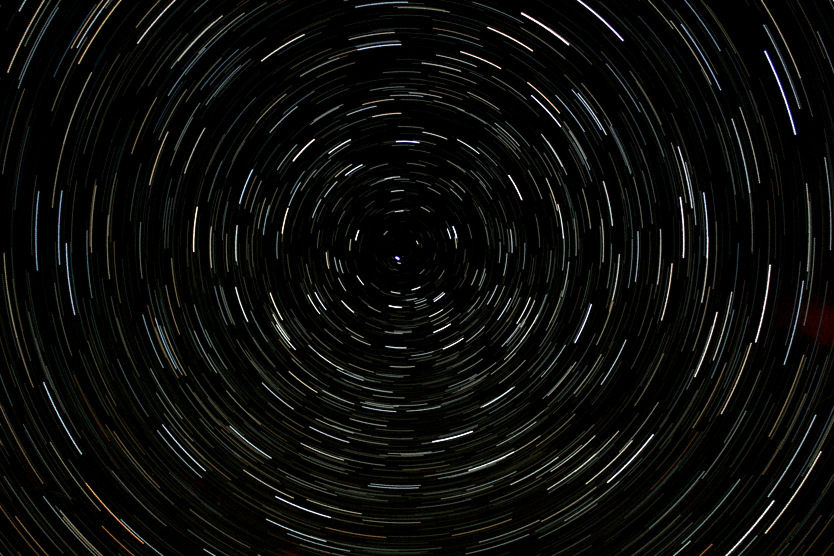
\includegraphics[width=\columnwidth]{img/star_trails_small.jpg}%
  \caption[Star motion around the northern celestial pole.]{Star motion
around the northern celestial pole. The image is com\-po\-sed of se\-ve\-ral
sub-frames, the total exposure time is about half an hour. Image by Robert
Vanderbei \citenum{Vanderbei:2012:LaPalma}.}
  \label{fig:star-trails}
\end{marginfigure}
\margincite{Vanderbei:2012:LaPalma}

\lettrine{O}{ur planet} is rotating, performing one full turn relative to the
sky in a stellar day of about 23 hours and 56 minutes
\cite[\ts12.2]{Allen:2000:Allen}. This poses a problem to photographers: Due to
the low light intensity of most astronomical objects, the exposure times for
astronomical images range from seconds to several hours. Without counteracting
the Earth's rotation, the stars travel long distances across a camera's image
sensor during exposure. Figure~\ref{fig:star-trails} shows an intentional
example of this effect.

Efforts to tackle this problem have lead to the development of specialized
mechanical devices, actuated \emph{telescope mounts}, that follow the stars'
motion. However, mechanical devices are never perfect. A slight imperfection in
the shape of a cog or a worm in the gear of a telescope mount leads to pointing
errors of usually several arcseconds\footnote[][3mm]{One arcsecond (\as) is the
3600$^\text{th}$ fraction of a degree.}. Taking into account the fine angular
resolution of typical imaging setups, this means several pixels of blur during a
long-exposure image.

The periodic error correction method based on Gaussian processes
(Chapter~\ref{ch:periodic-error-correction}) is suitable to address periodic
errors in telescope tracking. In this chapter we first describe the telescope
guiding problem (Section~\ref{sec:problem-statement}), and then apply the method
on both simulation and hardware experiments (Section~\ref{sec:pec-experiments}).

\section{The Telescope Problem}
\label{sec:problem-statement}

\begin{marginfigure}
\centering%
\footnotesize%
  \begin{tikzpicture}%
    \node [draw=none, inner sep=0] (t)
{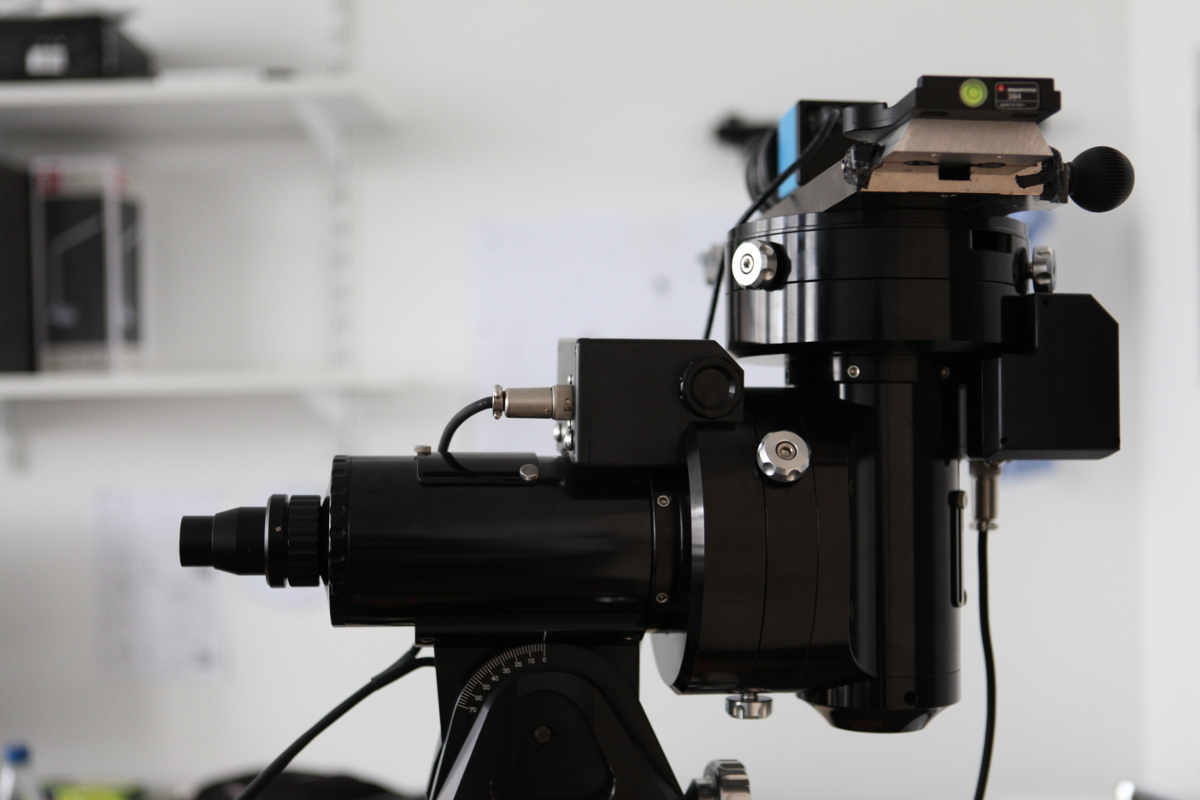
\includegraphics[width=\columnwidth]{img/equatorial_mount.jpg}};
    \draw [dgr, line width=1pt, transform canvas={yshift=-5.8mm}]
    (t.west) -- node[above, text=white]{RA} (t.east);
    \draw [dgr, dashed, line width=1pt, transform canvas={xshift=11.5mm}]
    (t.north) -- node[right, text=white]{Dec} (t.south);
  \end{tikzpicture}%
  \caption[Typical German equatorial mount.]{Typical German equatorial
mount. When used for astronomical imaging, the right ascension (RA) axis is
aligned with the Earth's rotational axis. The declination axis (Dec) is
necessary to be able to point at arbitrary
positions.}
  \label{fig:equatorial-mount}
\end{marginfigure}

Amateur telescope mounts for astronomical imaging are usually built in
equatorial design \margincite{Parker:2007:Making}%
\margincite{Beish:2001:Design}\citenum{Parker:2007:Making, Beish:2001:Design},
one such mount is shown in Figure~\ref{fig:equatorial-mount}. The mechanics is
designed in a way that the right ascension (RA) axis of the telescope mount is
aligned with the Earth's rotational axis when set up properly. This way, only
this axis has to be constantly in motion to follow the stars, which simplifies
the control problem. The telescope can now be modeled in the form of a linear
scalar model
\begin{align}
\label{eq:telescope-problem}
  \dot x(t) &= a_cx(t) + b_cu(t) + g(t),
\end{align}
where $a_c$ is the scalar dynamics, $b_c$ the scalar input gain and $g(t)$ a
scalar disturbance. As described in detail in
Chapter~\ref{ch:periodic-error-correction}, the disturbance is modeled with a
quasiperiodic Gaussian process regression model. It should be noted that in
practice, measurements of $\dot x(t)$ are generally not available and will be
approximated numerically, see also the experimental details in
Section~\ref{sec:pec-experiments}.

Existing \emph{periodic error correction} systems require careful system
identification by the user of the telescope, and still regularly lead to
unsatisfactory performance.

A challenge specific to this astronomical application is that state
measurements are performed by taking images of guiding stars
\margincite{Parker:2007:Making}\citenum[\ts1]{Parker:2007:Making}, which
requires relatively long exposure times, resulting in the measurement interval
reaching the order of magnitude of the error periodicity. This is precisely the
domain in which we expect to see utility from a periodic model.

The performance gain one can expect from the use of a periodic model for
feed-forward compensation depends on the sampling rate of the control system:
If the external error is slow compared to the measurement rate, a locally
linear model is sufficient. But if the external error is on the same time scale
as the measurement, it helps to use feed-forward control based on GP
predictions. With the presented approach it is even possible to choose the
control interval smaller than the actual measurement interval. See
Section~\ref{sec:pec-simulation} for a more detailed discussion.

\section{Experiments}
\label{sec:pec-experiments}

The presented method  was implemented for the telescope problem and evaluated
on different problems. After testing on a simulated telescope system, where the
performance under different measurement frequencies and under sensor failure was
analyzed, the proposed method was evaluated in an experiment on a real
telescope system, showing substantial improvements in control performance.

\subsection{Simulated System}
\label{sec:pec-simulation}

The period length of the periodic error in telescopes is relatively long. To
allow rapid prototyping, we designed a simulation system with dynamics similar
to a real telescope. Experiments have shown that the model can be simplified by
considering only the angular pointing error as state, measured relative to the
desired state. The pointing error can be influenced by an input velocity.
The resulting model is
\begin{equation}
  \dot x(t) = u(t) + g(t),
\end{equation}
with an unknown function $g(t)$ that is observed to be quasiperiodic.

Figure~\ref{fig:error_vs_dt} shows simulation results that empirically confirm
the intuition from Section~\ref{sec:problem-statement} that the benefit of
periodic prediction in control depends on the sampling rate. Using the numerical
simulation, we compare, for various sampling rates of the state,
\begin{itemize}
\item an MPC controller using the linear model
\eqref{eq:problem} with \mbox{$g(t) = 0\quad \forall t$}
\item two MPC controllers, both using a nonparametric, but fully stationary
(i.e.\ not periodic) GP model for $g$ with the square exponential covariance
function \eqref{eq:square-exp}; one of these models uses a length scale smaller
than the periodicity (\ie it can extrapolate periodic swings locally, but not
beyond one period); the other a length scale longer than the periodicity (\ie it
averages over the periodic variations)
\item two MPC controllers using instances of the periodic model for $g$; one in
which the hyperparameters are fixed to a good value a priori (amounting to the
assumption that the period of $g$ is known), the other using the full setup
described in Section~\ref{sec:gps_for_quasiperiodic_functions}, in which the
periodicity hyperparameter is learned by type-II maximum likelihood during
identification
\end{itemize}
Since we are only interested in the performance in the limit in this experiment,
all the controllers were run for an identification phase of 10 period lengths
to avoid artifacts from identification.
Figure~\ref{fig:error_vs_dt} shows RMS error, i.e.\ deviation of the state from
the origin, as a function of the sampling time. The RMS error is measured over
10 period lengths, starting after the identification phase. The discretization
time for the MPC is always set to \nicefrac{1}{100} of the period length, \ie to
1\unit{s}. Between measurements, the MPC controllers are operated in open-loop
mode, i.e. the control actions are obtained from the sequence of the last MPC
optimization.

\begin{figure}
\centering%
\footnotesize%
\inputTikZ{error_vs_dt_fine}%
\caption[Comparison of the RMS error at different sampling times.]{Comparison
of the RMS error at different sampling times (in simulation), for five different
prediction models: linear (\ref*{p:edt-lin}), square exponential with $\ell \ll
\lambda$ (\ref*{p:edt-se-short}), square exponential with $\ell \gg \lambda$
(\ref*{p:edt-se-long}), periodic with inferred $\lambda$ (\ref*{p:edt-per-inf})
and periodic with optimal $\lambda$ (\ref*{p:edt-per-opt}).
MPC control inputs are computed at the indicated sampling times, shown as a
fraction of the period length. The control rate is 1\unit{Hz} for every plot.
The MPC parameters were set to $\SC=10^2$ and $\CC=10^1$. The horizon length was
chosen such that the horizon covers the time until the next measurement.
Between measurements, the MPCs are operated in open-loop mode. $g(t)$ is set to
be a sine with fixed period $\lambda = 100\unit{s}$. }
\label{fig:error_vs_dt}
\end{figure}

The results demonstrate the intuition: For sampling times much smaller than
$\lambda$, the dynamics are locally linear, and all models achieve an error
close to zero. Their performance difference is only marginal (lower left in
Figure~\ref{fig:error_vs_dt}). For sampling times between about 10\unit{\%} and
80\unit{\%} of $\lambda$, the periodic model offers considerable benefits. When
the sampling times are close to, or larger than, the periodicity, the Nyquist
rate imposes limits on identifiability of the system, which adversely affects
the performance of the periodic nonparametric model. This shows that a broad
prior can lead to bad performance if only little data is available. On the
other hand, if $\lambda$ is known precisely, very good control is possible even
for sampling rates lower than $\lambda$. The parameter-inferring model
(\ref*{p:edt-per-inf}) in Figure~\ref{fig:error_vs_dt} represents the
performance of a system almost ignorant of $\lambda$ in the beginning: the
prior is very broad. One can expect prior information about $\lambda$ of
varying vagueness to give performance somewhere in the region between the
parameter-inferring model (\ref*{p:edt-per-inf}) and the optimal-parameter
model (\ref*{p:edt-per-opt}) in Figure~\ref{fig:error_vs_dt}.

The case where sampling rate and $\lambda$ are equal is special, since then $g$
appears to be constant in the measurements, and even the informed periodic
model can not learn the behavior of $g$. A weaker version of this effect is also
visible in the plot at a sampling rate of $\nicefrac{\lambda}{2}$. This
``selection bias'' affects all regression models, including the aperiodic ones.

\subsection{Evaluation of Fault Tolerance}
\label{sec:fault_tolerance}

A similar experiment was conducted to investigate the effect of missing
measurements on the performance of the controlled system.
Figure~\ref{fig:error_vs_darkness} shows the empirical results. The setup is the
same as in the experiment described before, but now the sampling time is fixed
to a value of $5\unit{s}$, while the period length is $100\unit{s}$. The length
of the horizon is set to $41$ time steps (\ie 205\unit{s}), covering more than
two full periods of the periodic effect, which is a realistic setting for a real
telescope.

After giving the system enough time to learn under regular output measurements,
no new data is used to update the GP model of $g(t)$, and no new state estimate
is available to the controller. This corresponds to a fault in the sensor (or
clouds in front of the camera in the telescope setting). The sensor does not
recover within the simulation time. Figure~\ref{fig:error_vs_darkness} shows
the performance of the different controllers, measured in terms of the RMS
error since the beginning of the fault, here at time $0$. In all controller
setups, the MPC control sequence can not be updated as there is no state
estimate available. For the following time steps without measurement, the MPC
therefore is operated in open-loop mode, \ie the control actions from the
control sequence computed at the time before the fault are used.

At the beginning of the failure (lower left of
Figure~\ref{fig:error_vs_darkness}), the performance of all methods is good,
since the effect of the periodic disturbance is still small. Over time, we see
the simple controller without prediction (\ref*{p:edt-lin}) slowly degrading.
Interestingly, the performance of the GP with square exponential kernel with
too long a length scale (\ref*{p:edt-se-long}) performs even worse than not
predicting $g(t)$ at all. This illustrates how critical the choice of the
hyperparameters is and that a wrong choice can even degrade the performance.
The model with sensible length scale (\ref*{p:edt-se-short}) performs
significantly better initially, but the extrapolation of the SE kernel degrades
quickly (see also Figure~\ref{fig:kernels} (a)) resulting in an overall
performance that is only slightly better than for the linear model.

With periodic predictions, in contrast, the controllers perform significantly
better during the fault. The periodic GP (\ref*{p:edt-per-inf}) is better than
the SE with short length scale, even if the period length is inferred and not
fixed at a good value. The RMS error for the GP with optimal parameter
$\lambda$ (\ref*{p:edt-per-opt}) is virtually zero and even a controller having
access to the true function $g(t)$ would therefore only show marginal
improvement. This analysis shows that the proposed combination of a periodic GP
model and MPC control is able to compensate temporary sensor failures and
maintain high control performance for locally periodic dynamic effects.

\begin{figure}%
\centering%
\footnotesize%
\inputTikZ{error_vs_darkness}%
\caption[Comparison of the RMS error after sensor failure.]{Comparison of the
RMS error after sensor failure (in simulation), for five different prediction
models: linear (\ref*{p:edt-lin}), square exponential with $\ell \ll \lambda$
(\ref*{p:edt-se-short}), square exponential with $\ell \gg \lambda$
(\ref*{p:edt-se-long}), periodic with inferred $\lambda$ (\ref*{p:edt-per-inf})
and periodic with optimal $\lambda$ (\ref*{p:edt-per-opt}). Sampling time and
discretization time of the MPC are both 5\unit{s}. The MPC parameters are set to
$\HL=41$, $\SC=10^2$ and $\CC=10^1$. After a training period, no new
measurements are available (``dark phase''). The MPC is operated in open-loop
mode. $g(t)$ is set to be a sine with fixed period $\lambda=100\unit{s}$.}
\label{fig:error_vs_darkness}
\end{figure}

\subsection{Hardware Experiment}
\label{sec:hardware}

We have tested our implementation on a physical system, a commercially
available \emph{Vixen} Sphinx telescope mount (Figure~\ref{fig:hardware}).
Without closed-loop control, this mount shows about 7\as~of RMS error after
correction for static drift. The error arises from the imperfect shape of the
cogs in the gear of this mount (Figure~\ref{fig:gearbox}). The imperfect shape
is not visible to the naked eye, see Figure~\ref{fig:hardware_measurement} (a)
for an uncontrolled measurement.

Because outdoor measurements are subject to random, time-varying effects like
weather conditions, we constructed a more reproducible experimental setup using
a second, high-precision gearless \emph{ASA} DDM60
\clearpage

\begin{figure}
\centering%
\footnotesize%
  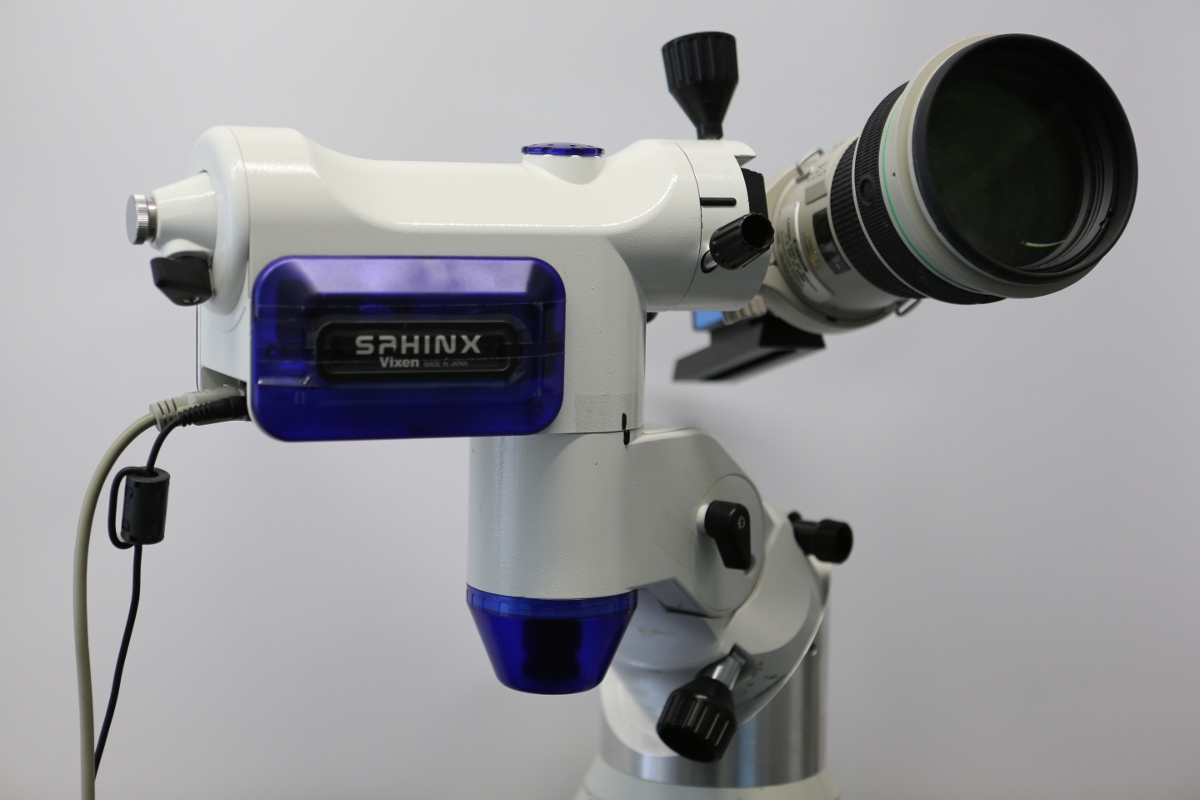
\includegraphics[width=\columnwidth]{img/mount_1200.jpg}%
  \caption[The telescope mount used for the tracking experiments.]{The telescope
mount used for the tracking experiments. On the right side is the camera lens
used as guiding telescope. A main telescope is not used for the tests.}%
  \label{fig:hardware}%
\end{figure}

\begin{figure}
\centering%
\footnotesize%
  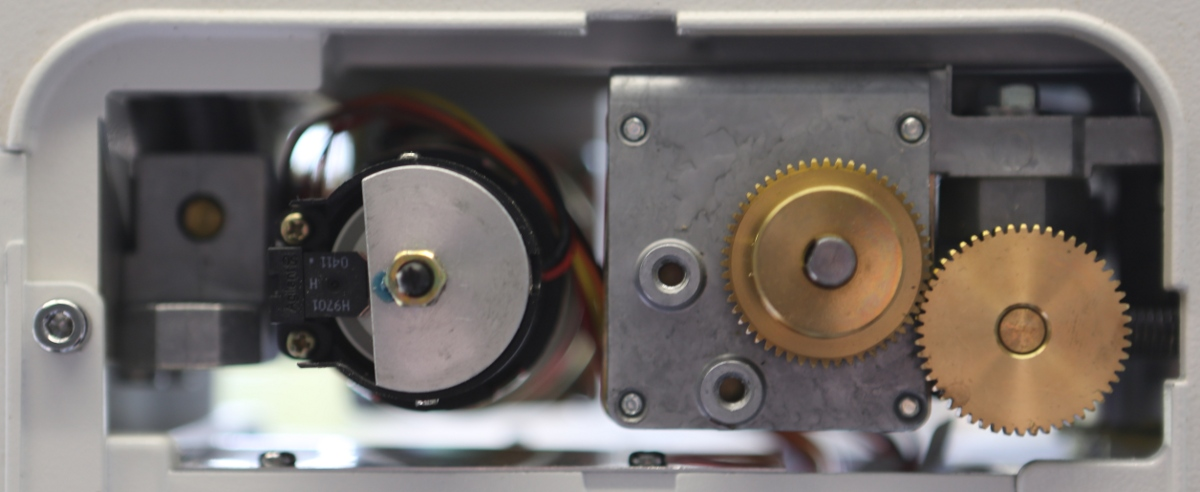
\includegraphics[width=\columnwidth]{img/gearbox_1200.jpg}%
  \caption[The gearbox of the telescope mount.]{The gearbox of the telescope
mount. One of the motors is visible on the left. The two cogs on the right
transmit the motor's rotation to a worm gear (not visible), which sits on the
same axis and thus has the same period. These cogs and the worm gear are the
likely
source of the periodic error.}%
  \label{fig:gearbox}%
\end{figure}

\noindent Pro telescope mount equipped
with a laser ``star'' as tracking reference (Figure~\ref{fig:gearless-mount}).
It has a typical tracking RMS error of about 0.4\as. The measurement is done
with a \emph{Canon} EF400DO lens on a \emph{The Imaging Source} DMK
41AU02.AS camera.

\begin{marginfigure}[3cm]
\centering%
\footnotesize%
  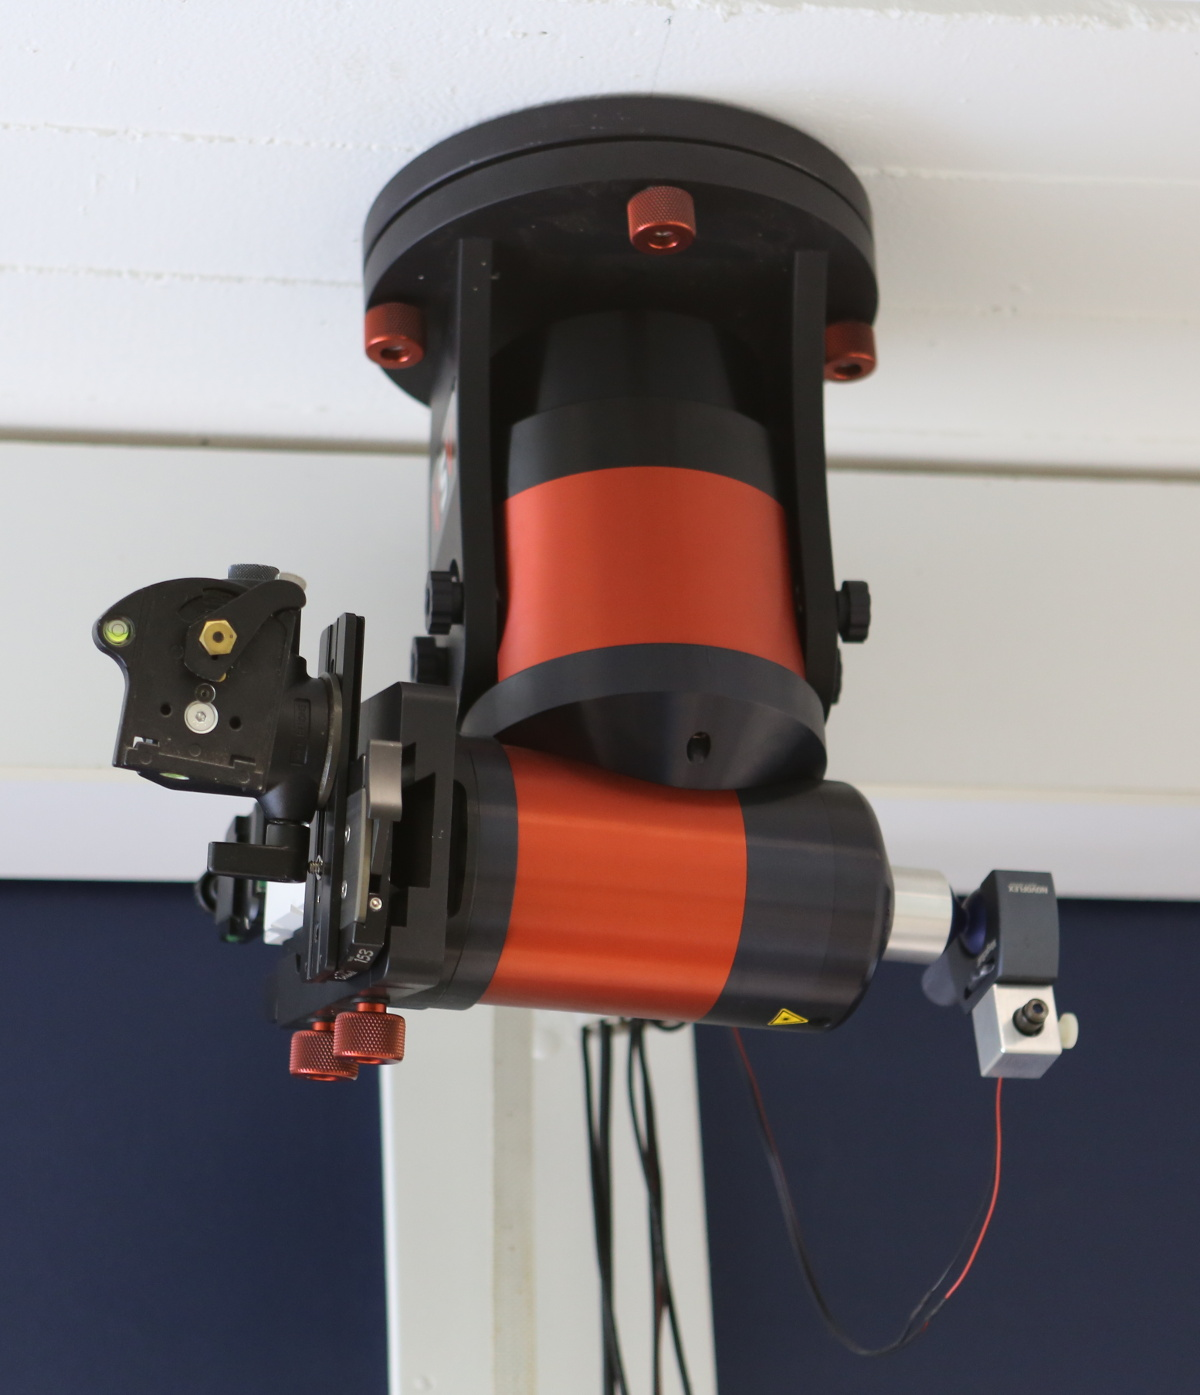
\includegraphics[width=\columnwidth]{img/mount_ceiling_1200.jpg}%
  \caption[The gearless \emph{ASA} DDM60 Pro telescope mount.]{The gearless
\emph{ASA} DDM60 Pro telescope mount, attached to the ceiling of our
laboratory.}%
  \label{fig:gearless-mount}%
\end{marginfigure}

For the hardware interaction, the open source ``PHD Guiding'' software package
is used. In the original implementation this software uses a proportional
controller with hysteresis to prevent direction switching. The telescope is
connected to the computer with a \emph{Shoestring Astronomy} GPUSB, a
device that sends pulse-width modulated signals to telescopes over a commonly
used 6-wire interface.

We altered the software to gain access to the measured displacement of the
camera image. The value is sent through a network socket to \textsc{Matlab},
with which the proposed controller was implemented to calculate the optimal
control signal. The control signal is sent back to the guiding software, which
\footnotetext[2]{The pixel resolution of our lens and camera
combination was determined with \texttt{nova.astrometry.net}
\citenum{Hogg.ea:2008:Automated}.}%
\margincite{Hogg.ea:2008:Automated}%
then passes it on to the telescope hardware. For plotting and
calculation of the RMS error, the measured displacement is converted from
pixels into arcseconds (\as) with an empirically determined conversion
factor\footnotemark.

For real-time implementation, algorithmic complexity is relevant. The
computational cost of the GP prediction scales cubically in the number of
data points. To bound computational cost, we limit the number of used data
points to 90 in a moving window fashion. This gives a sufficient coverage of
270\unit{s}, or about 3 periods of the short periodic component. Since
inference continuously runs in an extrapolation setting (see also
Figure~\ref{fig:kernels} (b)), this is sufficient for precise inference and
control.

For the prediction of the dynamics in the MPC framework, an ODE-solver is
employed to predict the tracking reference from the mean of the GP prediction.
This has manageable computational cost because the inference of a Gaussian
process is dominated by the initial one-time operation of inverting the Gram
matrix $K$ in $\mathcal{O}(\ND^3)$ time, while evaluating the mean function at
$M$ times only has cost $\mathcal{O}(M\ND)$.

The optimization of the hyperparameters is also an expensive part of this
algorithm. As the kernel Gram matrix has to be filled and inverted at every
evaluation of the objective function, the number of evaluations has to be kept
small at every sampling time. We use a numerical optimizer based on the BFGS
update
\margincite{Broyden:1969:new}%
\margincite{Fletcher:1970:new}%
\margincite{Goldfarb:1970:family}%
\margincite{Shanno:1970:Conditioning}%
\citenum{Broyden:1969:new, Fletcher:1970:new, Goldfarb:1970:family,
Shanno:1970:Conditioning}, a quasi-Newton algorithm that updates an
estimate of the inverse Hessian in each iteration. In the standard
implementation, the estimate of the Hessian obtained at one time step is
discarded after each individual call to the optimizer. For the use in the
control setting, we altered the algorithm so that the estimate of the inverse
Hessian is stored and used to initialize the optimizer's estimate at the next
sampling time. This makes it possible to do one iteration per sampling interval
(in a sense, threading the optimization algorithm into the learning algorithm).
This significantly reduces computation time.

The presented method was tested on two different setups, one with an MPC based
on the linear model only and one with the GP prediction for the periodic error
g(t). The test was run 3 times for 25\unit{min} each. Both the sampling and the
discretization time were set to 3\unit{s}. The horizon length was $\HL=10$; the
state and control weights were set to $\SC=10^2$ and $\CC=10^3$. The results of
these runs are shown in Table~\ref{tab:results-hardware}.

\begin{table}[ht]
{\centering
\footnotesize
\begin{tabular}{@{} r *4{r} @{}}
\toprule
          & Run 1  & Run 2  & Run 3  & {\bfseries Mean}   \\
\midrule
Plain MPC & 0.9839 & 1.0234 & 0.9353 & {\bfseries 0.9809} \\
GP-MPC    & 0.7365 & 0.7792 & 0.7605 & {\bfseries 0.7587} \\
\bottomrule
\end{tabular}
\vskip 0.1in
\caption[Experimental results from indoor telescope tracking.]{Experimental
results from indoor telescope tracking (RMS error, \as).}
\label{tab:results-hardware}
}
\end{table}

The RMS error drops by 22.64\unit{\%} through the use of GP predictions in this
hardware setup. Baseline measurements without movement showed about 0.25 to
0.35\as~of noise. The noise introduced by the stepper motor could not be
quantified with the current measurement system. Overall, the presented method
eliminated at least a third of the controllable error, after subtracting
baseline noise but without taking the stepper motor into account. This is a
good result in this domain, but could probably be further improved, which is
also visible through the weak residual structure visible in
Figure~\ref{fig:hardware_measurement} (c).

\begin{figure}
\centering
\footnotesize
\subfloat[Uncontrolled, RMS(e) =
6.533\as]{\inputTikZ{measurement_raw}
\label{fig:raw_measurement}}\\
\subfloat[Plain MPC, RMS(e) =
1.023\as]{\inputTikZ{measurement_plain_mpc}
\label{fig:plain_mpc_measurement}}\\
\subfloat[GP-MPC, RMS(e) = 0.779\as]{\inputTikZ{measurement_gp_mpc}
\label{fig:gp_mpc_measurement}}
\caption[State measurements from the indoor tracking experiment.]{State
measurements from the indoor tracking experiment: Without controller
(\refpoints{p:meas-raw}), where the highlighted
area (\ref*{p:meas-zoom}) shows the vertical range of the two other plots; for
plain MPC using only a linear model (\refpoints{p:meas-plain}); and for the
periodic Gaussian process based MPC (\refpoints{p:meas-gp}). The controlled
measurements' data are from run 2 of our experiments, which resulted in the
highest (worst) RMS error for both models (Table~\ref{tab:results-hardware}). }
\label{fig:hardware_measurement}
\end{figure}

Figure~\ref{fig:spectra} shows the power spectra of the measurements,
obtained from the Fourier transform. It is noticeable that the strong periodic
components near 100\unit{s} and near 500\unit{s}, as well as the constant
component are highly damped with the presented method.

\begin{figure}
\centering
\footnotesize
\subfloat[Plain MPC]{\inputTikZ{spectrum_plain_mpc}
\label{fig:spectrum_plain_mpc}}\\
\subfloat[GP-MPC]{\inputTikZ{spectrum_gp_mpc}
\label{fig:spectrum_gp_mpc}}
\caption[Power spectra from the indoor tracking experiment.]{Power spectra of
the measurements of Figure~\ref{fig:hardware_measurement}, plain MPC using only
a linear model (\ref*{p:spec-plain}), and periodic Gaussian process model based
MPC (\ref*{p:spec-gp}).} \label{fig:spectra}
\end{figure}


\section{Conclusion}

Telescope tracking requires high precision with low sampling rates. Therefore,
Gaussian process regression with a quasiperiodic prior is a well-suited
prediction framework for this application.

Numerical and hardware experiments confirm the intuitive result that the benefit
of periodic models depends on the relative size of state sampling and
disturbance frequencies. We showed that, even in cases where the gain of a
periodic prediction is only marginal during normal operation, these models are
beneficial when sensors fail temporarily. The presented method also shows
considerable increases in control performance, confirming the practical utility
of this framework.
